\documentclass[a4paper,10pt]{article}
\usepackage[slovene]{babel}
\usepackage[utf8]{inputenc}
\usepackage{lmodern}
\usepackage[T1]{fontenc}
\usepackage{lmodern}
\usepackage{amsfonts}
\usepackage{eurosym}
\usepackage{graphicx}
\usepackage{amssymb}
\usepackage{amsmath} 
\usepackage{qtree}
\usepackage{hyperref}
\usepackage{float}



\begin{document}
\title{ ISKANJE NAJBOLJŠE BLIŽNJICE V DREVESU \\ \large Projekt pri finančnem praktikumu \\ 9.skupina}
\author{Žiga Kodrič \and Katarina Kromar}
\maketitle

\section{Opis problema}
\subsection{Originalen}
Take an arbitrary tree T and assume that all the edge weights are 1. We want to add an edge e ("a shortcut") to T that minimizes the average distance between the vertices. This means that we want to choose the edge e such that the sum of the distances in T+e between all the pairs of vertices is minimized. We can find such an edge e by trying all possible edges. Check several random trees and see how much the average distance between vertices decreases when inserting the best shortcut. You may want to check also for two shortcuts (for small trees.)

\subsection{Opis problema}
Vzamemo drevo T in predpostavimo, da imajo vse povezave utež 1. Radi bi dodali neko povezavo e (bližnjico) na drevo T, ki bi minimizirala povprečno razdaljo med vozlišči. Torej bi radi izbrali tako povezavo e, da bo vsota razdalj v T+e med vsemi pari vozlišč minimizirana. Lahko poskusimo najti tako povezavo e tako, da poskusimo vse možne povezave. 
\\[0.5cm]
Ta postopek bova poskusila na nekaterih naključnih drevesih, kjer bova kodo oziroma funkcijo za generiranje takih drevesih poskusila najti na internetu. Poskusila bova ugotoviti, koliko se povprečna razdalja med vozlišči zmanjša, ko vključimo v drevo najboljšo bližnjico. Poskusila bova tudi z vključitvijo dveh bližnjic, kar pa bo seveda zaradi zahtevnosti programa potrebno poskusiti na manjših drevesih.

\section{Predstavitev grafov na računalniku in generiranje podatkov}
Grafe lahko predstavimo z matriko sosednosti ali pa s seznami sosednosti. Pri projektu bova uporabljala sezname, ker so bolj optimalni, saj zasedejo manj pomnilnika. Za vsako točko imamo torej seznam naslednikov in predhodnikov. Pri tem porabimo le $O(\mid V \mid + \mid E \mid)$ pomnilnika.
Če pregledamo vse sosede vozlišča $ u \in  V(G) $  porabimo $ O(\deg u)$ časa, za pregled vseh povezav pa $O(|V|+|E|)$.
Pri najinem projektu potrebujeva naključna drevesa. Poiskala bova kodo/funkcijo, ki bo vrnila naključno drevo na n točkah v obliki seznama sosedov.

\section{Osnovna ideja algoritma}
Algoritem sva si zamislila na naslednji način. Najprej bova zgenerirala naključno drevo na n točkah. Algoritem si bo nato izbral prvo točko. Tej točki bo dodal bližnjico in preko algoritma BFS izračunal vse možne razdalje, ter vrnil povprečje le teh. V nadaljnem delu sva ugotovila, da ne potrebujeva celotnega algoritma BFS, saj lahko uporabimo funkcijo v Sage-u \texttt{graph.average\_distance()}, ki izračuna povprečno razdaljo med vozlišči. Algoritem bo nato dodal naslednjo bližnjico (in prejšnjo seveda izbrisal), ter ponovno izračunal povprečje razdalj. V primeru, da bo povprečje manjše, bo shranil to bližnjico, v nasprotnem primeru pa jo bo ovrgel. Tako bo nadaljeval z računanjem dokler ne bo preveril vseh možnih bližnjic. Ko bo preveril vse možne bližnjice, bo nadaljeval na naslednjo točko in ponovno preveril vse možnosti. Algoritem se bo končal, ko bo preveril vse možnosti na vseh točkah. 
\newline
Program si bo hkrati zapisoval katere bližnjice je že pregledal. Če bo torej izračunal razdalje, ko bo dodal bližnjico $uv$,$u \in V(G),v\in V(G)$, bližnjice $vu$ ne bo ponovno pregledal.
\newline
Programirala bova v programskem jeziku Sage, ki je dostopen na spletni strani 
\url{https://cocalc.com/}
 in sicer zaradi enostavnosti generiranja naključnih dreves.

\section{Generiranje podatkov}
Za generiranje naključnih dreves bova uporabila programski jezik Sage in sicer z ukazom:
\begin{verbatim}
graphs.RandomTree(n).to_dictionary(),
\end{verbatim}
kar nam vrne naključno drevo na n vozliščih, pretvorjeno v seznam sosednosti. Vozlišča so označena od 0 do n-1.

\section{Algoritem}
%Najprej sva zaradi lažje predstave in enostavnosti vzela kar primer drevesa:
%
%\begin{verbatim} 
%graph = {"A": ["B", "D"],
%         "B": ["A","C"],
%         "C": ["B"],
%         "D": ["A","E"],
%         "E": ["D"]}
%\end{verbatim}
%
%Za lažjo predstavo ga narišimo:
%\Tree [.A [.B  C ] [.D  E ] ]
%\newline
%Da lahko narišemo drevo moramo naložiti paket \texttt{qtree}.
%\newline
Radi bi dobili povprečno razdaljo med vozlišči, zato definiramo funkcijo \texttt{dolzine(graph)}.
\begin{verbatim}
def dolzine(graph):
    s = 0
    graph = Graph(graph)
    s = graph.average_distance() #izračuna povprečno razdaljo med vozlišči
    return(s)
\end{verbatim}

Sedaj bi radi vključili bližnjico v \texttt{graph}, ki bi minimizirala povprečno razdaljo med vozlišči. Za vhod vzamemo graf, za izhod pa dobimo trojico, v katerem sta prva dva člena vozlišči, med katerima poteka bližnjica, tretji člen pa nam da minimalno povprečno razdaljo med vozlišči.

\begin{verbatim}
def bliznjica(graph):
    m = (0,0,99999999999999)
    povezave = [] #seznam preverjenih povezav
    k = list(graph.keys()) #seznam vozlišč
    for i in range(0,len(k)):
        for j in range(0,len(k)):
            #če povezave še ni in sta različni točki
            if k[j] not in graph.get(k[i]) and k[j] != k[i]:
                if (k[i],k[j]) not in povezave:
                    #dodamo nove povezave, graf neusmerjen
                    graph[k[i]].append(k[j])
                    graph[k[j]].append(k[i])
                    dol = dolzine(graph)  #izračunamo nove razdalje
                    graph[k[i]].remove(k[j])   #izbrišemo bližnjico
                    graph[k[j]].remove(k[i])
                    #dodamo bližnjico med že preverjene
                    povezave.append((k[i],k[j]))
                    povezave.append((k[j],k[i]))

                    if dol < m[2]:   #preverimo če je nova bližnjica boljša
                        m = (k[j],k[i], dol)
    return(m)
\end{verbatim}

Poglejmo, kako je, če dodamo 2 bližnjici v drevo. Funkcija je sestavljena na podoben način kot za eno bližnjico. Preveri vse možne povezave, hkrati pa preverja, če je to povezavo že pregledala. 
\small
\begin{verbatim}
def dve_bliznjici2(graph):
    m2 = (0,0,0,0,99999999999999)
    preverjene = []
    g = []
    k = list(graph.keys())
    for i in range(0, len(k)):
        for j in range(0,len(k)):
            for s in range(0, len(k)):
                for l in range(0,len(k)):
                    if k[s] not in graph.get(k[i]):
                        if k[l] not in graph.get(k[j]):
                            if k[i] != k[s] :
                                if k[j] != k[l]:
                                    if k[i] != k[j]:
                                        if (k[i],k[s]) != (k[j],k[l]):
                                            if (k[s],k[i]) != (k[l],k[j]) and 
				(k[s],k[i]) != (k[j],k[l]) and(k[i],k[s]) != (k[l],k[j]):
# (zamaknjeno samo zaradi lažjega prikaza)
                                                if (k[i], k[s],k[j],k[l]) not in preverjene:
                                                    graph[k[i]].append(k[s])
                                                    graph[k[j]].append(k[l])
                                                    graph[k[s]].append(k[i])
                                                    graph[k[l]].append(k[j])
                                                    dol = dolzine(graph)
                                                    graph[k[i]].remove(k[s])
                                                    graph[k[j]].remove(k[l])
                                                    graph[k[s]].remove(k[i])
                                                    graph[k[l]].remove(k[j])
                                                    preverjene.append((k[i],k[s],k[j],k[l]))
                                                    preverjene.append((k[s],k[i],k[j],k[l]))
                                                    preverjene.append((k[i],k[s],k[l],k[j]))
                                                    preverjene.append((k[s],k[i],k[l],k[j]))
                                                    if dol < m2[4]:
                                                        m2 = (k[i],k[s],k[j],k[l],dol)
                                                    g.append((k[i], k[s],k[j],k[l]))
    return(m2)
\end{verbatim}
\normalsize
Ker pa je funkcija za iskanje dveh bližnjic časovno zahtevna, naju je zanimalo, če lahko poiščemo dober približek dveh najboljših bližnjic. Zato sva sestavila funkcijo \texttt{najboljsa\_bliznjica1()}. Najprej poiščemo prvo bližnjico z že napisanim programom \texttt{bliznjica}, jo dodamo v drevo in nato z istim postopkom poiščemo še drugo bližnjico na novem grafu. Koda nam vrne peterico: prva dva člena sta vozlišči, med katerima poteka prva bližnjica, druga dva vozlišči med katerima poteka druga bližnjica ter peti člen minimalna povprečna razdalja med vozlišči. V nadaljevanju sva tudi analizirala, kako dober približek bližnjic nam vrne ta funkcija.

\begin{verbatim}
def dve_bliznjici1(graph, prva_bliznjica):
    k = list(graph.keys())
    najboljsi_bliznjici = (0,0,0,0,0)
    prva = prva_bliznjica           #Prvo bližnjico že poznamo
    graph[prva[0]].append(prva[1])    #Dodamo v drevo
    graph[prva[1]].append(prva[0])
    druga = bliznjica(graph)          #Poiščemo drugo bližnjico
    najboljsi_bliznjici = (prva[0],prva[1],druga[0],druga[1],druga[2])
    graph[prva[0]].remove(prva[1])   #Izbrišemo bližnjico iz grafa
    graph[prva[1]].remove(prva[0])
    return(najboljsi_bliznjici)
\end{verbatim}


%V primeru, ko na drevo, ki smo ga izbrali zgoraj, dodamo le eno bližnjico, nam funkcija \texttt{bliznjica} vrne \texttt{('C', 'A', 1.25) }, torej je najboljša bližnjica med C in A in sicer v tem primeru pride povprečna razdalja med vozlišči 1.25. Če dodamo dve bližnjici v drevo, dobimo \texttt{('C', 'A', 'E', 'A', 1.0)}, torej dodamo še bližnjico med A in E, ter tako dobimo minimalno povprečno razdaljo med vozlišči 1.0.

\section{Primeri naključnih dreves}

Uporabimo kodo v Sage-u:
\begin{verbatim}
drevo =graphs.RandomTree(10)
drevo.show()
drevo.to_dictionary()
\end{verbatim}
Vrne nam drevo:$ \lbrace 0: [3], 1: [5], 2: [7, 8], 3: [0, 4, 5], 4: [3], \\ 5: [1, 3, 6], 6: [5, 7], 7: [2, 6, 9], 8: [2], 9: [7] \rbrace$
\begin{center}
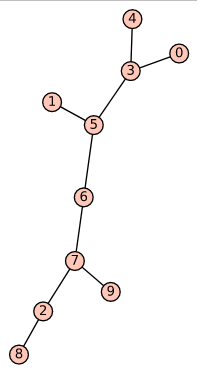
\includegraphics[scale = 0.6]{graf1}\\ 
\scriptsize{\textit{Slika 1: } Naključno drevo na 10 vozliščih.}
\end{center}
Povprečna razdalja med vozlišči je 3.444, najboljša bližnjica, ki minimizira povprečno razdaljo med vozlišči je med 7 in 0, povprečna razdalja med vozlišči je tedaj 2.0. Če vključimo še eno bližnjico in sicer med 1 in 0, dobimo povprečno razdaljo med vozlišči 1.778.
\\[0.5cm]
Poskusimo sedaj na malo večjih drevesih in podatke zapišimo v tabelo:
\\[0.5cm]
\begin{tabular}{ |p{3cm}||p{3cm}|p{3cm}|p{3cm}|  }
 \hline
 \multicolumn{4}{|c|}{Naključna drevesa} \\
 \hline
 Število vozlišč& Povprečna razdalja med vozlišči &Povp. razd. med vozlišči, če vključimo 1 bližnjico&Povp. razd. med vozlišči, če vključimo 2 bližnjici\\
 \hline
 10   & 2.711    &2.311&   2.089\\
 30 &6.609 & 4.676& 4.156\\
 50    &8.286 & 5.757& 5.295\\
 70&10.248&7.274&6.216\\
 100&  11.223  & 8.905&7.420\\
 
 \hline
\end{tabular}

\section{Časovna zahtevnost}
Opazimo, da koda pri drevesih s 100 vozlišči dela že kar počasi, saj mora preveriti vse povezave. Poglejmo časovno zahtevnost algoritma. Funkcija sprejme argumente n, m in \texttt{stevilo\_bliznjic}. n je število vozlišč, m pa število ponovitev. Če je \texttt{stevilo\_bliznjic} enako 1, funkcija uporabi funkcijo \texttt{bliznjica()}, če 2 \texttt{dve\_bliznjici1()} in 3 \texttt{dve\_bliznjici2()}. Funkcija vrne potreben čas.
\begin{verbatim}
def casovna_zahtevnost(n,m,stevilo_bliznjic):
    import time
    funkcija = [bliznjica, dve_bliznjici1, dve_bliznjici2][stevilo_bliznjic-1]
    start = time.time()
    for i in xrange(m):
        if funkcija == dve_bliznjici1:
            drevo=graphs.RandomTree(n).to_dictionary()
            funkcija(drevo,bliznjica(drevo))
        else:
            funkcija(graphs.RandomTree(n).to_dictionary())
    konec = time.time()
    return(konec-start)
\end{verbatim}
Poglejmo nekaj primerov za lažjo predstavo:
\begin{verbatim}
casovna_zahtevnost(200,1,1)      57.819862842559814
casovna_zahtevnost(10,100,2)     0.9815769195556641
casovna_zahtevnost(10,100,3)     52.104007959365845
casovna_zahtevnost(20,100,1)     3.494917869567871
casovna_zahtevnost(120,130,1)    1285.5924899578094
\end{verbatim}
Časovna zahtevnost glede na število vozlišč:
\begin{verbatim}
casovna_vozlisca = []
for i in range(4,31):
    # drevesa z od 4 do 30 vozlišči, ponovimo 100x, 1 bližnjica
    casovna_vozlisca.append(casovna_zahtevnost(i,100,1)) 
casovna_vozlisca
\end{verbatim}
\begin{center}
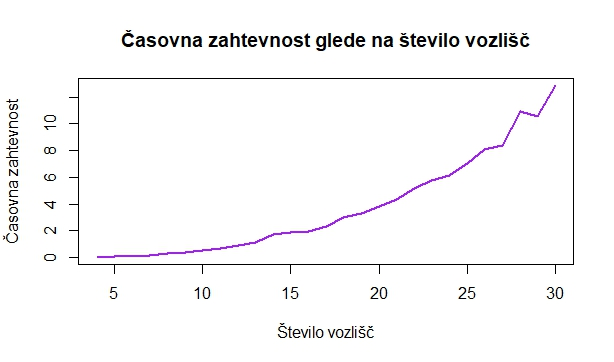
\includegraphics[scale = 0.8]{casovna}\\ 
\scriptsize{\textit{Graf 1: } Časovna zahtevnost algoritma glede na število vozlišč .}
\end{center}
\section{Približek drugi bližnjici}
Iskanje dveh najboljših bližnjic se je izkazalo za časovno zelo zahtevno. Zato naju je zanimalo ali obstaja način, da najdemo zadovoljiv približek. Zato sva se odločila, da pogledava kako dobri bližnjici najde program, ki namesto dveh bližnjic naenkrat išče dvakrat najboljšo bližnjico. Torej najde prvo najboljšo bližnjico, jo doda v drevo in nato v tem grafu poišče najboljšo bližnjico. Primerjala sva razlike povprečnih razdalj v grafih z različnimi števili vozlišč. Dobila sva naslednjo tabelo: \newline
\begin{table}[H]
\centering
\caption{Razlike povpr. razdalj z različnimi št. vozlišč}
\label{my-label}
\begin{tabular}{lllllllllllll}
Razlika razdalje/Št. vozlišč & 4 & 5 & 6 & 7     & 8     & 9 & 10 & 11 & 12 & 13    & 14 & 15 \\
Razlika razdalje             & 0 & 0 & 0 & 0,048 & 0,036 & 0 & 0  & 0  & 0  & 0,075 & 0  & 0 
\end{tabular}
\end{table}

Če generiramo 50 dreves z 12 vozlišči in pogledamo razliko povprečnih razdalj, dobimo, da je v povprečju razlika le 0,04. V primeru 50 dreves z 20 vozlišči ponovno dobimo, da je napaka enaka 0,04. \newline
Poglejmo si še časovno zahtevnost funkcij. Pogledala sva si, koliko časa potrebujeta funkciji za izračun najboljših bližnjic na enakih drevesih z od 4 do 15 vozlišči. Dobila sva tabelo: 
\begin{table}[H]

\caption{Časovna zahtevnost}
\label{my-label}
\begin{tabular}{@{\hspace{-2cm}}llllllllllll}
                        & 4      & 5      & 6      & 7      & 8      & 9      & 10    & 11    & 12   & 13    & 14    \\ 
najboljsa\_\\
bliznjica1() & 0.0008 & 0.0012 & 0.0023 & 0.0035 & 0.0056 & 0.0095 & 0.012 & 0.015 & 0018 & 0.026 & 0.04  \\ 
najboljsa\_\\
bliznjica2() & 0.0009 & 0.0037 & 0.0123 & 0.0356 & 0.094  & 0.24   & 0.65  & 1.29  & 2.68 & 5.3   & 10.15 \\ 
\end{tabular}
\end{table}



Če zgeneriramo 10 grafov s 15 vozlišči bo funkcija \texttt{ dve\_bliznjici1()} v povprečju porabila 0.037 sekunde, medtem ko funkcija \texttt{dve \_bliznjici2()} porabi 18.9 sekund. Izkaže se torej, da se nam sploh v večjih grafih bolj splača uporabiti fukncijo \texttt{dve\_bliznjici1()}, saj je napaka relativno majhna, hkrati pa je funkcija veliko hitrejša.
\section{Ugotovitve}
 Koliko se povprečna razdalja med vozlišči zmanjša, ko vključimo v drevo najboljšo bližnjico?
\newline

Pogledamo, za koliko se spremeni povprečna razdalja. Funkcija \texttt{ razlika\_ razdalj } sprejme argumenta n, m ter \texttt{ stevilo\_bliznjic}. Označimo n kot število vozlišč drevesa, m število ponovitev in \texttt{stevilo\_bliznjic} (1 ali 2) število bližnjic, ki jih dodamo v graf. Vrne par, kjer prvo število predstavlja povprečno razdaljo v drevesu brez bližnjice in drugo v drevesu z bližnjico. 
\begin{verbatim}
def razlika_razdalj(n,m, stevilo_bliznjic):
    i = 0
    seznam_razdalj_dve = []
    seznam_razdalj = []
    seznam_razdalj_bliznjica = []
    if stevilo_bliznjic == 1:
        while i < m:
            drevo1 = graphs.RandomTree(n).to_dictionary()
            seznam_razdalj.append(dolzine(drevo1))
            seznam_razdalj_bliznjica.append(bliznjica(drevo1)[2])
            i += 1
        return((sum(seznam_razdalj)/m,sum(seznam_razdalj_bliznjica)/m))
    if stevilo_bliznjic == 2:
        while i < m:
            drevo1 = graphs.RandomTree(n).to_dictionary()
            seznam_razdalj.append(dolzine(drevo1))
            prva_bliznjica = bliznjica(drevo1)
            seznam_razdalj_bliznjica.append(prva_bliznjica[2])
            seznam_razdalj_dve.append(dve_bliznjici1(drevo1,prva_bliznjica)[4])
            i += 1
        return((sum(seznam_razdalj)/m,sum(seznam_razdalj_dve)/m))
    else:
        return("Funkcija kot stevilo_bliznjic sprejema števila 1 ali 2")
\end{verbatim}

Razlika razdalj, če imamo 10 vozlišč z 1 bližnjico, postopek pa ponovimo 100-krat:  (3.099, 1.989) (prva številka pove, kolikšna je povprečna razdalja v drevesu, druga pa kolikšna je povprečna razdalja, če vključimo najboljšo bližnjico).
\newline
Imamo 30 vozlišč, postopek ponovimo 70x, vključimo 1 bližnjico:
\begin{verbatim}
razlika_razdalj(30,70,1),
\end{verbatim}
vrne nam recimo (5.720, 3.471).
Če imamo 15 vozlišč, postopek ponovimo 50x, vključimo 2  bližnjici: (3.587, 1.984).
\\[0.5cm]
Spreminjanje razdalje glede na število vozlišč. Gledamo, za koliko se spremeni povprečna razdalja v drevesu z od 4 do 30 vozlišči na 100 ponovitev, če dodajamo eno bližnjico:
\begin{verbatim}
razdalje_vozlisca = []
for i in range(4,31):
    m = razlika_razdalj(i,100,1)
    razdalje_vozlisca.append(m)
razdalje_vozlisca
\end{verbatim}
Poskusimo narisati v programu R:
\begin{center}
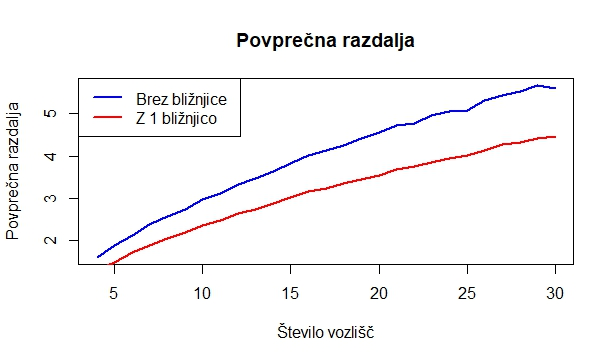
\includegraphics[scale = 0.75]{povp_razd}\\ 
\scriptsize{\textit{Graf 2: } Povprečna razdalja med vozlišči ter če vključimo eno bližnjico.}
\end{center}


Ugotovila sva, da čas, ki ga porabimo za iskanje bližnjice v drevesu eksponentno raste s številom vozlišč, kar je tudi pričakovan rezultat. Pričakovano je tudi, da več kot je ponovitev, daljši je čas izvajanja algoritma, prav tako traja dlje, če namesto ene bližnjice iščemo dve.
\newline
Opazila sva tudi, da se povprečna razdalja med vozlišči, ko vključimo eno bližnjico, zmanjša in sicer razlika med povprečno razdaljo med vozlišči v drevesu in povprečno razdaljo z eno bližnjico je večja, ko večamo število vozlišč. 
\newline
Ko gledamo, koliko v odstotkih je ta sprememba, ugotovimo, da je okoli 80\%, torej, ko dodamo bližnjico, se v povprečju zmanjša povprečna razdalja med vozlišči za okoli 80\%.
\newline
Naš primer (razlika v \%):
\begin{verbatim}
82.55934   79.53340   80.27466   78.90967   79.62269   80.00404   79.67778
79.52475   79.39057   78.85268   79.16993   79.14651   78.53694   78.42466
78.72314   78.21699   77.77059   78.25767   78.97192   77.59482   78.14983
79.05210   77.54679   78.61552   78.03397   78.08158   80.03028
\end{verbatim}
\end{document}
